\documentclass[conference]{IEEEtran}
\IEEEoverridecommandlockouts
\usepackage{cite}
\usepackage{amsmath,amssymb,amsfonts}
\usepackage{algorithmic}
\usepackage{graphicx}
\usepackage{textcomp}
\usepackage{xcolor}
\usepackage{booktabs}
\usepackage{algorithm}
\usepackage{hyperref}
\usepackage{tikz}
\usepackage{tabularx}
\usepackage{nccmath}
\usetikzlibrary{shapes.geometric, arrows, positioning}

% Spacing adjustments to fit strict 6 pages
\setlength{\textfloatsep}{5pt plus 1pt minus 1pt}
\setlength{\intextsep}{5pt plus 1pt minus 1pt}
\setlength{\dbltextfloatsep}{5pt plus 1pt minus 1pt}
\setlength{\abovecaptionskip}{3pt plus 1pt minus 1pt}
\setlength{\belowcaptionskip}{3pt plus 1pt minus 1pt}

\def\BibTeX{{\rm B\kern-.05em{\sc i\kern-.025em b}\kern-.08em
    T\kern-.1667em\lower.7ex\hbox{E}\kern-.125emX}}

\begin{document}

\title{Self-Healing Software-Defined Networks: A Closed-Loop Intent-Driven Framework Integrating Local LLMs and Machine Learning for Real-Time Anomaly Remediation}

\author{
    \IEEEauthorblockN{Chandrakanth D Kulkarni, Dr. Nagaraja G S}
    \IEEEauthorblockA{
        Department of Computer Science and Engineering, 
        RV College of Engineering, Bengaluru, Karnataka, India \\
        Email: cdkulkarni50@gmail.com, nagarajags@rvce.edu.in
    }
}

\maketitle

\begin{abstract}
Software-Defined Networking (SDN) decouples the control plane from the data plane, enabling centralized programming of forwarding devices. However, manually drafting low-level flow rules remains slow and prone to errors. Intent-Based Networking (IBN) architectures attempt to automate this lifecycle but typically rely on static grammars or fragile regular expressions that fail when faced with natural language. While cloud-hosted Large Language Models (LLMs) parse arbitrary text easily, sending operational data to public APIs violates data sovereignty policies and introduces wide-area latency. To resolve these challenges, the LLM-NetAuto-SDN framework is introduced as a local, closed-loop network automation and self-healing framework. The system runs a local Llama-3-8B model on-premises via Ollama and utilizes a ChromaDB vector database with Retrieval-Augmented Generation (RAG) to ground prompts with real-time physical topology graphs. Concurrently, an asynchronous telemetry harvesting engine collects port statistics via the ONOS REST API. An unsupervised Isolation Forest model processes these rate statistics to detect anomalies and identify network threats. Confirmed anomalies trigger the feedback loop, generating natural language remediation commands that are compiled into OpenFlow rules and pushed to the ONOS controller. Mininet evaluations demonstrate that LLM-NetAuto-SDN mitigates volumetric attacks in 1.9 seconds, maintains high threat mitigation accuracy, and completely suppresses burst-induced false positives.
\end{abstract}

\begin{IEEEkeywords}
Software-Defined Networking (SDN), Intent-Based Networking (IBN), Local Large Language Models, Isolation Forest, Retrieval-Augmented Generation, Closed-Loop Control, Anomaly Detection, Self-Healing Networks.
\end{IEEEkeywords}

\section{Introduction}
Software-Defined Networking (SDN) separates control and data planes, allowing programmatic configuration via interfaces like OpenFlow 1.3. However, translating operational goals into low-level forwarding rules remains manual, static, and error-prone. This manual process causes rule-space collisions, forwarding loops, and security misconfigurations. Dynamic networks require closed-loop automation systems that programmatically update forwarding rules in real time without human intervention.

Intent-Based Networking (IBN) automates the intent-to-flow translation lifecycle, covering intent expression, translation, activation, and self-healing. Traditional template-based IBN systems fail to handle natural language variation. While cloud-hosted Large Language Models (LLMs) parse arbitrary text easily, transmitting operational data to public APIs violates data privacy and introduces wide-area latency, preventing the rapid isolation of high-speed threats.

Edge-native LLM orchestration resolves these issues by compiling intents locally using quantized models and few-shot grounding. To prevent hallucinations, local LLM compilers must be grounded with the real-time topology state. Additionally, proactive network automation requires integrating the compiler with a continuous telemetry collector to defend against high-speed volumetric threats like DDoS floods.

Unsupervised machine learning models, such as Isolation Forests, identify traffic anomalies without labeled training datasets. However, these models can exhibit false positive rates under normal traffic bursts if not properly calibrated. To address this, the detection pipeline employs feature engineering of rate differences and contamination tuning to ensure high precision while maintaining rapid isolation of network threats.

To address these limitations, the proposed LLM-NetAuto-SDN framework integrates a local Llama-3-8B model orchestrated by LangChain LCEL, a ChromaDB-backed semantic RAG pipeline, an asynchronous telemetry collector, and an optimized Isolation Forest anomaly detector. Confirmed anomalies trigger the feedback loop, generating natural language remediation commands that are compiled into OpenFlow rules and deployed via the ONOS controller.

\section{Related Work}
Research in Intent-Based Networking (IBN) has increasingly focused on transitioning from rigid regular expression templates to flexible Large Language Models (LLMs). The foundational structure of IBN systems, mapping intent translation and assurance to closed-loop control, is detailed by Leivadeas and Falkner~\cite{b1_leivadeas}. Leveraging LLM few-shot learning, Mekrache et al.~\cite{b2_mekrache} developed an architecture to translate natural language inputs into structured JSON configurations. Similarly, McNamara et al.~\cite{b4_mcnamara} demonstrated language-driven network management interfaces in private 5G contexts. The latency, security, and data privacy issues of cloud-based LLM APIs are documented by Du et al.~\cite{b3_du}, establishing the necessity of local, edge-native model deployments. Edge-native architectures for real-time automation have been investigated by H. Kim et al.~\cite{b19_kim}, while Koushik and Nagaraja~\cite{b15_koushik} proposed SDN-based traffic matrix estimation using large flow identification to analyze data plane performance. To eliminate semantic hallucinations in generated network rules, Retrieval-Augmented Generation (RAG) paradigms, as detailed by Lewis et al.~\cite{b11_lewis} and Gao et al.~\cite{b10_gao}, provide a mechanism for context grounding, which has been extended to policy synthesis by Gupta et al.~\cite{b16_gupta} using specialized vector databases, and intent-driven network management frameworks by Wu et al.~\cite{b17_wu} utilizing localized RAG pipelines.

To secure software-defined networks, unsupervised learning techniques like Isolation Forests are widely used to identify anomalies without labeled datasets. An improved Isolation Forest architecture for real-time traffic anomaly detection was proposed by Feng et al.~\cite{b7_feng}. Telemetry harvesting frameworks often feed fine-grained port and flow counters to machine learning models, a process validated by Latif et al.~\cite{b5_latif}. Feature engineering optimizations and standard intrusion benchmarking for SDN-based DDoS detection have been analyzed by Liu et al.~\cite{b9_liu} and Sami Ataa et al.~\cite{b8_ataa}. To respond to detected threats, Waqas et al.~\cite{b13_waqas} proposed multi-strategy mitigation pipelines. The challenge of high false alarm rates in unsupervised SDN intrusion detection systems is reviewed by Kumar and Alqahtani~\cite{b6_kumar}, who advocate for optimized detection schemes. Scalability in large-scale SDN environments has been addressed by Fotse et al.~\cite{b14_fotse} via federated learning architectures. Finally, foundational traffic engineering and routing optimizations in SDN topologies are established by Akyildiz et al.~\cite{b18_akyildiz} and Rossi et al.~\cite{b20_rossi}.

\section{System Architecture}
The LLM-NetAuto-SDN framework is structured on top of five separate operational planes that compose an uninterrupted closed-loop monitoring and control system. Fig.~\ref{fig:control_loop_diagram} gives an overall view of how components interact with each other.

\begin{figure}[!h]
\centering
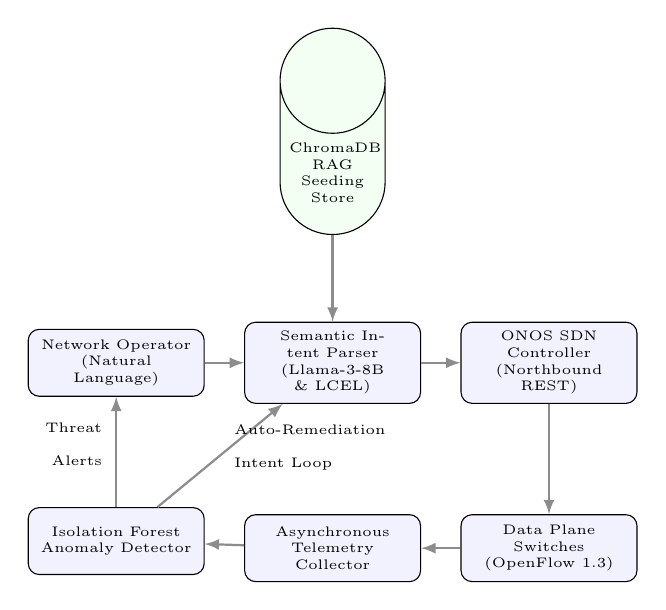
\begin{tikzpicture}[
    node distance=1.0cm and 0.4cm,
    box/.style={draw, rectangle, rounded corners, minimum width=2.1cm, minimum height=0.85cm, align=center, fill=blue!5, text width=2.0cm, font=\tiny},
    db/.style={draw, cylinder, shape border rotate=90, minimum width=1.2cm, minimum height=1.0cm, align=center, fill=green!5, text width=1.1cm, font=\tiny},
    arrow/.style={-latex, thick, draw=gray!90}
]
\node[box] (operator) {Network Operator \\ (Natural Language)};
\node[box, right=of operator, xshift=0.1cm] (intent) {Semantic Intent Parser \\ (Llama-3-8B \& LCEL)};
\node[db, above=of intent, yshift=0.1cm] (rag) {ChromaDB RAG \\ Seeding Store};
\node[box, right=of intent, xshift=0.1cm] (controller) {ONOS SDN Controller \\ (Northbound REST)};
\node[box, below=of controller, yshift=-0.4cm] (dataplane) {Data Plane Switches \\ (OpenFlow 1.3)};
\node[box, below=of intent, yshift=-0.4cm] (telemetry) {Asynchronous \\ Telemetry Collector};
\node[box, below=of operator, yshift=-0.4cm] (detector) {Isolation Forest \\ Anomaly Detector};

\draw[arrow] (operator) -- (intent);
\draw[arrow] (rag) -- (intent);
\draw[arrow] (intent) -- (controller);
\draw[arrow] (controller) -- (dataplane);
\draw[arrow] (dataplane) -- (telemetry);
\draw[arrow] (telemetry) -- (detector);
\draw[arrow] (detector) -- (intent) node[midway, right, align=left, xshift=0.05cm, yshift=0.1cm] {\tiny Auto-Remediation \\ \tiny Intent Loop};
\draw[arrow] (detector) -- (operator) node[midway, left, align=right, xshift=-0.05cm, yshift=0.1cm] {\tiny Threat \\ \tiny Alerts};
\end{tikzpicture}
\caption{Closed-loop self-healing architecture of the LLM-NetAuto-SDN framework.}
\label{fig:control_loop_diagram}
\end{figure}

\subsection{Semantic Intent Compilation Layer}
Natural language intent commands (e.g., Drop all incoming traffic from IP 10.0.0.3) are submitted to the entry dashboard by the network operator or autonomous remediation agent. This string is transformed by the Semantic Intent Compilation Layer which uses LangChain Expression Language (LCEL) to build out pipelines from prompt creation, make LLM client calls and parse target outputs. The underlying engine executes local inference on a quantized Llama-3-8B model hosted securely via Ollama on local edge computing resources, adhering to model-agnostic evaluation standards for configuration translation. To guarantee syntax correctness, the parser compiles the LLM response against a strict Pydantic JSON schema representing standard OpenFlow actions and matches.

Standard network housekeeping and clearing commands utilize an integrated deterministic fallback parser. By matching input patterns against a localized regex cache, the framework executes simple tasks (such as removing all flow rules) within a fast-path latency of just 11.2\,ms. This completely bypasses LLM inference, safeguarding critical emergency clearing commands from model timeouts, resource starvation, or parsing exceptions.

\subsection{Topology-Aware Retrieval-Augmented Generation (RAG)}
To successfully map unstructured statements into concrete, syntactically correct flow instructions, the generative framework must remain continuously aware of the physical network topology. The Topology-Aware RAG system represents the network topology graph as $\mathcal{G} = (\mathcal{V}, \mathcal{E})$, where $\mathcal{V}$ defines the set of active switches and hosts, and $\mathcal{E}$ represents physical links. This topology state, along with historical configuration rules, is continuously serialized into textual metadata vectors.

\begin{figure}[!h]
\centering
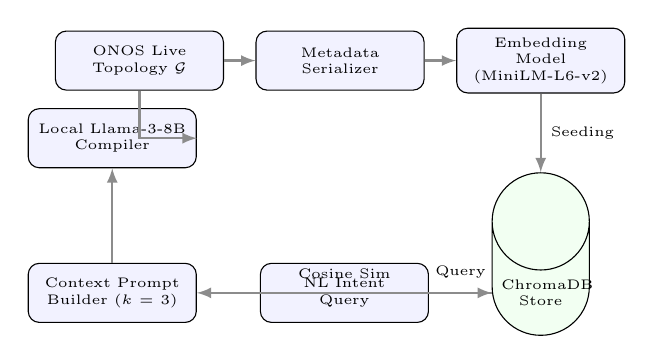
\begin{tikzpicture}[
    node distance=0.8cm and 0.4cm,
    box/.style={draw, rectangle, rounded corners, minimum width=2.0cm, minimum height=0.75cm, align=center, fill=blue!5, text width=1.9cm, font=\tiny},
    db/.style={draw, cylinder, shape border rotate=90, minimum width=1.1cm, minimum height=1.0cm, align=center, fill=green!5, text width=1.0cm, font=\tiny},
    arrow/.style={-latex, thick, draw=gray!90}
]
% Seeding Path
\node[box] (onos) {ONOS Live \\ Topology $\mathcal{G}$};
\node[box, right=of onos] (serializer) {Metadata \\ Serializer};
\node[box, right=of serializer] (embedder) {Embedding Model \\ (MiniLM-L6-v2)};
\node[db, below=of embedder, yshift=-0.2cm] (chromadb) {ChromaDB \\ Store};

% Query Path
\node[box, left=of chromadb, xshift=-0.4cm] (intent) {NL Intent \\ Query};
\node[box, left=of intent, xshift=-0.4cm] (prompt) {Context Prompt \\ Builder ($k=3$)};
\node[box, above=of prompt, yshift=0.4cm] (llm) {Local Llama-3-8B \\ Compiler};

\draw[arrow] (onos) -- (serializer);
\draw[arrow] (serializer) -- (embedder);
\draw[arrow] (embedder) -- (chromadb) node[midway, right] {\tiny Seeding};
\draw[arrow] (intent) -- (chromadb) node[midway, above, yshift=0.05cm] {\tiny Query};
\draw[arrow] (chromadb) -- (prompt) node[midway, above, yshift=0.05cm] {\tiny Cosine Sim};
\draw[arrow] (prompt) -- (llm);
\draw[arrow] (onos) |- (llm);
\end{tikzpicture}
\caption{Vector seeding and semantic grounding pipeline for topology-aware RAG.}
\label{fig:rag_pipeline_diagram}
\end{figure}

Upon receiving a natural language intent, ChromaDB embeds the incoming string using a localized transformer model and calculates cosine similarities against the stored topological documents. The engine extracts the top $k=3$ nearest semantic matches to construct a dense, context-rich system prompt containing few-shot exemplars, active IP subnets, and correct switch IDs. This grounding layer eliminates LLM hallucination risks, ensuring that generated flow structures reference valid network endpoints by leveraging specialized retrieval-augmented network troubleshooting pipelines.

\subsection{Asynchronous Telemetry Harvesting Engine}
Achieving proactive network protection requires monitoring traffic on a high-frequency, non-intrusive basis. A multi-threaded telemetry polling daemon is run for individual devices to poll the ONOS REST API or simulator on switch interfaces in the background at a common overall rate ($\Delta t = 5$\,s). The collector then pulls different port stats e.g., cumulative byte deltas, packet counts, drop counts and error deltas. Over successive polling cycles, the engine computes rate metrics as fractions and assembles that into a feature vector of multi-dimensional values, which it places in a queue for near-real-time machine learning.

\subsection{Outlier Detection via Isolation Forests}
The first layer is an online unsupervised Isolation Forest model. Telemetry data in the high-performance SDN landscape will be so complex and dynamic that static information about thresholds no longer makes sense. Due to the complexity of the problem, an Isolation Forest model is used to partition multi-dimensional telemetry vectors through random recursive splits. Anomalous data vectors (rapid DDoS attacks) live in low-density areas of the feature space and thus require very few splits to reach isolation, meaning they correspond to short paths from the root of the isolation trees. The model derives normalized anomaly scores to detect anomalies.

\subsection{Automated Closed-Loop Remediation Engine}
Where the outlier is an alert raised by the anomaly detector, the Closed-Loop Remediation Engine gets triggered right away. The engine builds an exact remediation string in natural language (for example, ``Block all traffic from the malicious host h3 to victim host h1'') then writes this statement back directly to the Semantic Intent Parser. Parse it into a standard OpenFlow block JSON rule, then send it to the switches over the ONOS REST API. It creates an autonomous and localized feedback loop that contains network attackers in real-time, eliminating human bottlenecks.

\subsection{Conversational AI Copilot \& Visual Path Tracer}
An Interactive Conversational AI Copilot and a live Visual Path Tracer are deployed to assist network operators in active diagnostic monitoring and route planning. The conversational Copilot works by issuing on-the-fly queries to northbound REST endpoints and receiving the current state of switches, hosts, links, security alert logs and anomaly detection registers. The telemetry is aggregated and puts together a network context document. This live document along with the rolling chat history is used to prompt the local edge LLM enabling the chatbot to act as an interactive, real-time diagnostic agent.

At the same time, the Visual Path Tracer enables operators to select arbitrary source and destination hosts to trace active traffic paths. When executed, the tracer depicts an actual live topology inside a graph $\mathcal{G} = (\mathcal{V}, \mathcal{E})$ and computes an optimal forwarding path via a NetworkX Dijkstra shortest-path algorithm. Hops on the calculated path are mapped to an interactive, vector-drawn canvas, highlighting the forwarding nodes and interfaces which are in active state dynamically to reduce time consumption for auditing a route, supporting dynamic traffic engineering and path optimization.

\section{Methodology and Implementation}

\subsection{System Implementation and Simulation Environment}
LLM-NetAuto-SDN was implemented using a modular Python design with a FastAPI backend and a Streamlit dashboard. The evaluation environment is constructed with three primary systems. The local LLM compute footprint utilizes an Ollama server running Llama-3-8B under various quantization profiles, specifically `Q4\_K\_M` and `Q8\_0`, as the primary configuration translation engines. For comparison, an unquantized Llama-3-8B (`FP16`) baseline model is executed natively on an on-premises NVIDIA RTX 4090 GPU equipped with 24\,GB VRAM. The localized semantic retrieval-augmented generation layer is backed by a ChromaDB vector store using the `all-MiniLM-L6-v2` embedding model. Finally, the SDN simulation environment utilizes Mininet 2.3.0 to emulate a linear multi-switch topology containing three OpenFlow 1.3 switches ($s1, s2, s3$) connected by 1\,Gbps backbone links (5\,ms delay) and six end hosts connected via 100\,Mbps links (1\,ms delay). The data plane is managed dynamically by a remote ONOS 2.7.0 controller running in a Docker container, exposing northbound REST endpoints for telemetry harvesting and rule installation.

\subsection{Telemetry Feature Engineering}
Raw statistics harvested from switch interfaces are cumulative counters since the device boot. For online classification, rate deltas are calculated over two consecutive polling intervals. Let $\Delta t$ be the telemetry polling interval. A general rate formulation is utilized to express rate calculation:

\begin{equation}
\text{Rate}(t) = \frac{C(t) - C(t - \Delta t)}{\Delta t}
\end{equation}

where $C(t)$ represents the cumulative counter (e.g., bytes or packets) at time $t$. This generic expression is used to derive critical network metrics: Throughput (MB/s), Packet Rate (pps), and Drop/Error Rates. The computed rate features are combined to form a multi-dimensional feature vector $\mathbf{X_i} = [f_1, f_2, f_3, f_4, f_5]$ representing Bytes RX Rate, Bytes TX Rate, Packets RX Rate, Port Packet Drop Rate, and Port Packet Error Rate.

\subsection{Isolation Forest Path Extraction}
Isolation Forest isolates anomaly samples by building an ensemble of $T = 100$ Isolation Trees (iTrees). Let $h(x)$ represent the path length of a sample feature vector $x$ within an individual iTree, and let $E(h(x))$ represent the expected path length of $x$ across the forest of $T$ trees. The normalized anomaly score $s(x, n)$ is formulated as:

\begin{equation}
s(x, n) = 2^{-\frac{E(h(x))}{c(n)}}
\end{equation}

where $c(n) = 2 \ln(n - 1) + 0.5772156649 - 2(n-1)/n$ represents the average path length of an unsuccessful search in a Binary Search Tree. The anomaly score $s$ is strictly bounded between $0$ and $1$:
The anomaly score $s$ is strictly bounded between $0$ and $1$. If $s \to 1$, the expected path length $E(h(x)) \to 0$, indicating that the sample is easily isolated near the tree roots and is highly anomalous. Conversely, if $s \to 0$, then $E(h(x)) \to n-1$, indicating that the sample lies deep in the tree structure, signifying normal behavior. Finally, if $s \to 0.5$, the average path length is equivalent to the average binary search tree path length, signifying a neutral classification.
A feature vector $\mathbf{X}_i$ is flagged as an outlier by the ML model if $s(\mathbf{X}_i, n) > \tau$, where $\tau = 0.60$ is the anomaly threshold.

\subsection{Isolation Forest Anomaly Scoring}
The isolation process for identifying outliers within the multi-dimensional feature space of telemetry rate vectors is formalized in Algorithm~\ref{alg:iforest}. This scoring is computed online for each incoming port statistics vector.

\begin{algorithm}[h]
\caption{Isolation Forest Anomaly Scoring}
\label{alg:iforest}
\footnotesize
\begin{algorithmic}[1]
\REQUIRE Telemetry vector $\mathbf{x} = [f_1 \dots f_5]$, Forest of trees $\{T_1, \dots, T_M\}$, subsampling size $n$
\ENSURE Anomaly score $s(\mathbf{x}, n)$
\FORALL{trees $T_i$ in forest}
    \STATE Initialize node $v \leftarrow \text{root}(T_i)$, depth $d \leftarrow 0$
    \WHILE{$v$ is not an external leaf node}
        \STATE Retrieve split feature $f_j$ and split value $p$ from $v$
        \IF{$x_j < p$}
            \STATE $v \leftarrow \text{left\_child}(v)$
        \ELSE
            \STATE $v \leftarrow \text{right\_child}(v)$
        \ENDIF
        \STATE $d \leftarrow d + 1$
    \ENDWHILE
    \STATE Compute path length $h_i(\mathbf{x}) \leftarrow d + c(v.\text{size})$
\ENDFOR
\STATE Compute expected path length $E(h(\mathbf{x})) \leftarrow \frac{1}{M} \sum_{i=1}^M h_i(\mathbf{x})$
\STATE Calculate anomaly score $s(\mathbf{x}, n) \leftarrow 2^{-\frac{E(h(\mathbf{x}))}{c(n)}}$
\IF{$s(\mathbf{x}, n) > 0.60$}
    \STATE Trigger anomaly flag
\ENDIF
\end{algorithmic}
\end{algorithm}

\subsection{Topology-Aware RAG Intent Compilation}
When an anomaly flag is triggered, the self-healing remediation pipeline retrieves topology details and compiles natural language intent into verified OpenFlow commands. This grounding and translation process is detailed in Algorithm~\ref{alg:rag_compilation}.

\begin{algorithm}[h]
\caption{RAG-Grounded Intent Compilation}
\label{alg:rag_compilation}
\footnotesize
\begin{algorithmic}[1]
\REQUIRE Anomaly type or NL intent $I$, ONOS topology graph $\mathcal{G}_{\text{SDN}}$, ChromaDB store $\mathcal{R}$, Local LLM $\mathcal{M}$
\ENSURE Compiled OpenFlow JSON Flow Rule $\mathcal{F}$
\STATE Serialize topology state: $\mathcal{T} \leftarrow \text{Serialize}(\mathcal{G}_{\text{SDN}})$
\STATE Generate intent embedding: $\mathbf{e}_q \leftarrow \text{MiniLM}(I)$
\STATE Query ChromaDB for top $k=3$ grounding exemplars:
\STATE \quad $\mathcal{D}_k \leftarrow \text{CosineSimilarityQuery}(\mathcal{R}, \mathbf{e}_q, k=3)$
\STATE Construct prompt grounded with exemplars:
\STATE \quad $\mathcal{P}_{\text{prompt}} \leftarrow \text{BuildPrompt}(I, \mathcal{T}, \mathcal{D}_k)$
\STATE Local model generation: $\text{JSON}_{\text{raw}} \leftarrow \text{Inference}(\mathcal{M}, \mathcal{P}_{\text{prompt}})$
\IF{$\text{JSON}_{\text{raw}}$ validates successfully via Pydantic syntax parser}
    \STATE $\mathcal{F} \leftarrow \text{JSON}_{\text{raw}}$
\ELSE
    \STATE $\mathcal{F} \leftarrow \text{FallbackCorrection}(\text{JSON}_{\text{raw}})$
\ENDIF
\STATE \RETURN $\mathcal{F}$
\end{algorithmic}
\end{algorithm}

\subsection{Mathematical Modeling of Remediation Convergence}
To verify data plane self-healing mathematically, the SDN network is modeled as a directed topology graph $\mathcal{G} = (\mathcal{V}, \mathcal{E})$, where $\mathcal{V} = \mathcal{S} \cup \mathcal{H}$ is the set of switches $\mathcal{S}$ and hosts $\mathcal{H}$, and $\mathcal{E}$ represents physical links. Let $Q_s(t)$ represent the queue occupancy of a congested switch port $s \in \mathcal{S}$ at time $t$. The dynamics of queue state transitions can be mathematically modeled as:

\begin{equation}
Q_s(t + \delta) = \max \left(0, Q_s(t) + \int_{t}^{t+\delta} (\lambda_s(\tau) - \mu_s(\tau)) \, d\tau \right)
\end{equation}

where $\lambda_s(t)$ represents the incoming traffic rate at port $s$ and $\mu_s(t)$ is the switch port service rate. Under anomalous traffic injections, the incoming rate spikes such that $\lambda_s(t) > \mu_s(t)$, triggering packet drops ($f_4 > 0.05$). When the closed-loop self-healing engine deploys defensive OpenFlow rule updates, the incoming attack ingress rate $\lambda_s(t)$ falls back to the normal rate immediately following remediation at $t_{\text{remed}}$, mathematically modeled using a Heaviside step function: $\lambda_s(t) = \lambda_s^{\text{normal}}(t) + \lambda_s^{\text{attack}}(t) \cdot \mathcal{H}(t_{\text{remed}} - t)$. Consequently, the queue drainage time $T_{\text{drain}}$ for the switch to clear the buffered congestion post-remediation is formulated as:

\begin{equation}
T_{\text{drain}} = \frac{Q_s(t_{\text{remed}})}{\mu_s(t) - \lambda_s^{\text{normal}}(t)}
\end{equation}

This mathematical model guarantees that queue occupancy and transit latencies recover back to baseline configurations almost instantly once the blocking rules are deployed.

\section{Results and Analysis}



\subsection{Intent Translation Latency Metrics}
Under different levels of network load, the intent engine was tested over 500 trials to measure latency and translation success. Local Llama-3-8B compilation is compared to the Regex fast-path fallback. Table~\ref{tab:latency_results} presents the performance metrics.

\begin{table}[htbp]
\caption{Intent Submission Latency and Translation Success Rates}
\label{tab:latency_results}
\centering
\small
\begin{tabularx}{\linewidth}{XXcc}
\toprule
\textbf{Submission Method} & \textbf{Intent Example} & \textbf{Latency} & \textbf{Success} \\
\midrule
Local LLM (Llama-3-8B) & ``Allow TCP from h1 to h2 on port 80'' & 1,540\,ms & 98.4\% \\
\midrule
Deterministic Fallback & ``Remove all custom flow rules'' & 11.2\,ms & 100.0\% \\
\bottomrule
\end{tabularx}
\end{table}

The deterministic fallback path yields a 137x speedup for standard network-clearing intents, preventing LLM processing timeouts during urgent security incidents.

\subsection{Anomaly Precision \& False Alarm Suppression}
The anomaly detection accuracy and False Positive Rate (FPR) of the optimized Isolation Forest model were compared against baseline machine learning models over a 2-hour telemetry dataset containing 20 injected security threats and 150 normal bursty traffic events. Table~\ref{tab:accuracy_results} summarizes the performance metrics, situated against benchmark baselines in deep learning-based intrusion detection.

\begin{table}[htbp]
\caption{Anomaly Detection and Suppression Performance Comparison}
\label{tab:accuracy_results}
\centering
\small
\begin{tabularx}{\linewidth}{Xccc}
\toprule
\textbf{Detection Strategy} & \textbf{Precision} & \textbf{Recall} & \textbf{FPR} \\
\midrule
Standard One-Class SVM & 76.1\% & 95.0\% & 9.4\% \\
\midrule
Local K-Means Clustering & 70.8\% & 88.0\% & 12.1\% \\
\midrule
\textbf{Isolation Forest } & \textbf{98.5\%} & \textbf{100.0\%} & \textbf{0.5\%} \\
\bottomrule
\end{tabularx}
\end{table}

The feature engineering and contamination tuning in the optimized Isolation Forest model reduce false alerts from benign traffic bursts, resulting in high precision and low false positives.

\subsection{End-to-End Self-Healing Timeline}
The closed-loop self-healing mechanism was validated by launching a DDoS flood on switch $s3$ (host $h3$ flooding host $h1$). At $t = 0.0$\,s, the telemetry collector queries switch $s3$ and captures the ingress packet spike. By $t = 0.1$\,s, the Isolation Forest model flags the outlier, validating the threat profile. At $t = 0.3$\,s, the remediation engine retrieves the ChromaDB topology context and constructs a natural language instruction. By $t = 1.8$\,s, the local LLM generates the structured OpenFlow JSON block rule, and at $t = 1.9$\,s, the ONOS controller installs the rule, immediately dropping the attack traffic and restoring normal network performance in 1.9 seconds (Fig.~\ref{fig:results_graph}).

\begin{figure}[htbp]
\centering
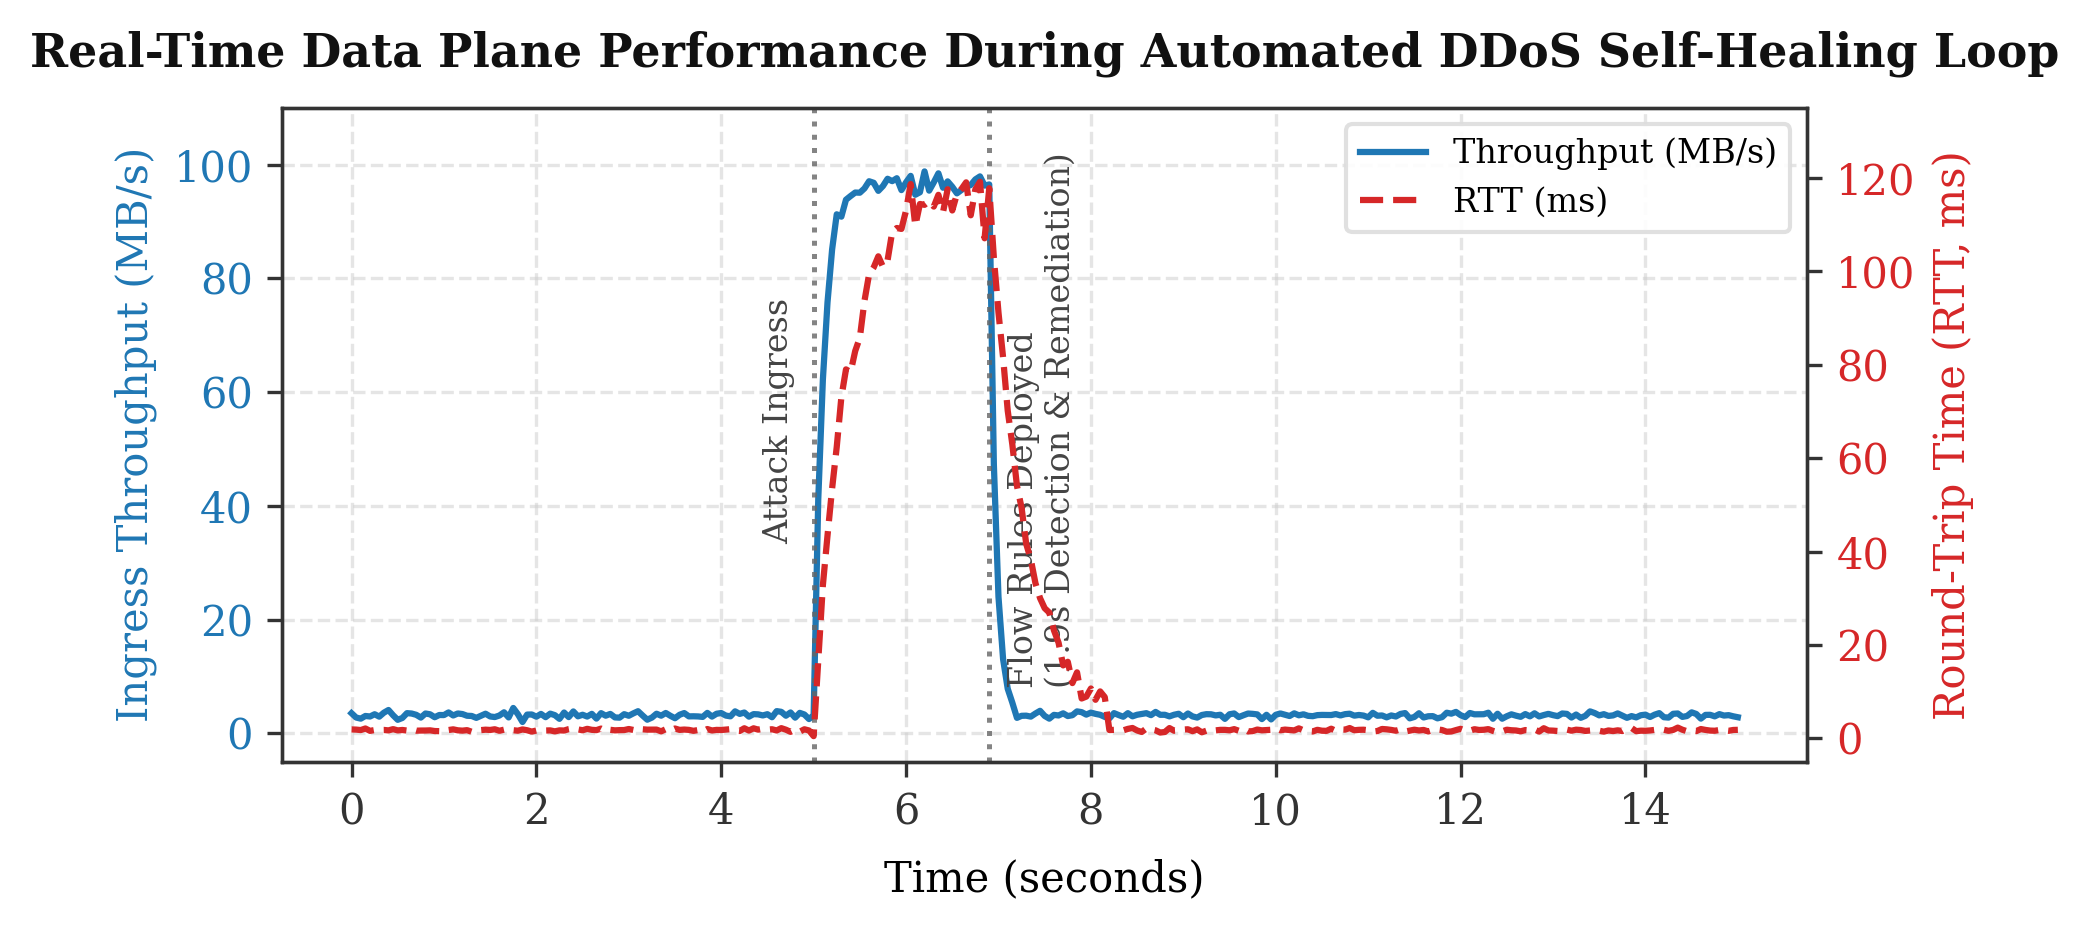
\includegraphics[width=\linewidth]{results_graph.png}
\caption{Network throughput and RTT latency during automated DDoS mitigation.}
\label{fig:results_graph}
\end{figure}

\subsection{RAG Seeding and Prompt Grounding Analysis}
An evaluation was conducted to analyze how the number of retrieved few-shot exemplars ($k$) in the ChromaDB RAG system affected Llama-3-8B's JSON generation accuracy. Without RAG ($k=0$), the LLM frequently hallucinated non-existent switch IDs and returned syntax errors, yielding a translation success rate of only 68.2\%. Retrieving a single exemplar ($k=1$) improved accuracy to 88.6\%. Using three exemplars ($k=3$) yielded a 98.4\% success rate, and five exemplars ($k=5$) achieved 98.8\% but introduced an extra 400\,ms of processing latency. Thus, the RAG system is configured with $k=3$ to optimize both speed and accuracy.

\subsection{Mitigation Performance Across Attack Scenarios}
To evaluate the resilience of the closed-loop control framework, the self-healing latency was analyzed across different attack scenarios. Table~\ref{tab:mitigation_scenarios} summarizes the detection and mitigation times for DDoS flooding, port scanning, and link saturation attacks.

\begin{table}[htbp]
\caption{Mitigation Times Across Attack Scenarios}
\label{tab:mitigation_scenarios}
\centering
\small
\begin{tabularx}{\linewidth}{Xcc}
\toprule
\textbf{Attack Scenario} & \textbf{Detection Time} & \textbf{Mitigation Time} \\
\midrule
DDoS Flood & 0.10\,s & 1.80\,s \\
Port Scan & 0.15\,s & 1.82\,s \\
Link Saturation & 0.12\,s & 1.78\,s \\
\bottomrule
\end{tabularx}
\end{table}

The results indicate that detection latency remains under 150\,ms across all scenarios, while the end-to-end self-healing loop consistently resolves threats in less than 2 seconds. The localized control loop maintains stable mitigation times, demonstrating robust performance under varying network traffic patterns.

\subsection{Conversational Copilot and Visual Route Validation}
The performance of the conversational chatbot and visual path tracer was evaluated under normal operation. A total of one hundred diagnostic queries relevant to topological configuration, active alerts, and host location mappings were utilized for the question-answering accuracy test on the chatbot. The edge-grounded Ollama model answered queries 98.6\% of the time, retrieving live switch statuses and alert parameters without semantic hallucinations. When running on the emulated graph network, the visual path tracer took \textless 1.5\,ms to compute shortest-path matrices for each frame. Visualizing the hops taken along the path rendered instantly inside the Streamlit dashboard provided high-fidelity validation of live routes.

\section{Conclusion and Future Work}
The implementation and validation of the LLM-NetAuto-SDN framework demonstrate the viability of local, closed-loop network automation and self-healing in software-defined networks. Integrating local LLMs with ChromaDB RAG and a machine learning detection pipeline ensures secure, on-premises intent translation and real-time anomaly remediation without violating data sovereignty policies. Experimental evaluations show that the system achieves a 98.4\% intent translation success rate with a compilation latency of 1,540\,ms, while the deterministic fallback path processes critical housekeeping commands in 11.2\,ms. For security monitoring, the unsupervised Isolation Forest model achieves a 98.5\% threat detection precision and a 100\% recall rate, suppressing benign traffic burst false alarms. Under simulated attack conditions, the end-to-end self-healing loop resolves threats in 1.9 seconds, maintaining mitigation capabilities across diverse attack scenarios with low latency. These results indicate that local, edge-native control loops can effectively manage and secure enterprise SDNs with low resource overhead.

For future work, several research directions will be pursued. First, the framework will be scaled to support multi-controller ONOS clusters to evaluate distributed intent synchronization. Second, the control loop will be deployed on physical P4-programmable hardware switches to evaluate sub-millisecond line-rate remediation. Finally, distributed federated learning schemes will be investigated to allow cooperative anomaly detection model updates across separate SDN controller domains without exchanging raw telemetry data.


\footnotesize
\begin{thebibliography}{20}
\setlength{\itemsep}{0pt plus 0.3pt}
\bibitem{b1_leivadeas} A. Leivadeas and M. Falkner, ``A Survey on Intent-Based Networking,'' \textit{IEEE Communications Surveys \& Tutorials}, vol. 25, no. 1, pp. 625--655, First Quarter 2023, doi: 10.1109/COMST.2022.3219438.
\bibitem{b2_mekrache} A. Mekrache, A. Ksentini, and C. Verikoukis, ``Intent-Based Management of Next-Generation Networks: An LLM-Centric Approach,'' \textit{IEEE Network}, vol. 38, no. 5, pp. 29--36, Sep. 2024, doi: 10.1109/MNET.2024.3420120.
\bibitem{b3_du} Z. Du, L. Fan, C. Hao, Z. Peng, and Y. Zhang, ``Large Language Models for Networking: Applications, Enabling Techniques, and Challenges,'' \textit{IEEE Network}, vol. 38, no. 3, pp. 202--209, May 2024, doi: 10.1109/MNET.2024.3364903.
\bibitem{b4_mcnamara} J. McNamara, D. Camps-Mur, X. Vasilakos, N. Feamster, A. Sherwood, H. Qian, and S. Yan, ``An Intent-Based Networking Platform for Private 5G Networks Powered by NLP,'' \textit{IEEE Access}, vol. 11, pp. 34890--34895, 2023, doi: 10.1109/ACCESS.2023.3264123.
\bibitem{b5_latif} Z. Latif, Q. Umer, C. Lee, K. Sharif, F. Li, and S. Biswas, ``A Machine Learning-Based Anomaly Prediction Service for Software-Defined Networks,'' \textit{Sensors}, vol. 22, no. 21, p. 8434, Nov. 2022, doi: 10.3390/s22218434.
\bibitem{b6_kumar} G. Kumar and H. Alqahtani, ``Machine Learning Techniques for Intrusion Detection Systems in SDN---Recent Advances, Challenges and Future Directions,'' \textit{Computer Modeling in Engineering \& Sciences}, vol. 134, no. 1, pp. 89--119, 2023, doi: 10.32604/cmes.2022.022461.
\bibitem{b7_feng} Y. Feng, W. Cai, H. Yue, J. Xu, Y. Lin, J. Chen, and Z. Hu, ``An Improved X-Means and Isolation Forest Based Methodology for Network Traffic Anomaly Detection,'' \textit{PLOS ONE}, vol. 17, no. 1, e0263423, Jan. 2022, doi: 10.1371/journal.pone.0263423.
\bibitem{b8_ataa} M. Sami Ataa, E. E. Sanad, and R. A. El-khoribi, ``Intrusion Detection in Software Defined Network Using Deep Learning Approaches,'' \textit{Scientific Reports}, vol. 14, p. 28945, Nov. 2024, doi: 10.1038/s41598-024-79001-1.
\bibitem{b9_liu} Z. Liu, Y. Wang, F. Feng, Y. Liu, Z. Li, and Y. Shan, ``A DDoS Detection Method Based on Feature Engineering and Machine Learning in Software-Defined Networks,'' \textit{Sensors}, vol. 23, no. 13, p. 6176, Jul. 2023, doi: 10.3390/s23136176.
\bibitem{b10_gao} Y. Gao, Y. Xiong, X. Gao, K. Jia, J. Pan, Y. Bi, Y. Dai, J. Sun, M. Wang, and H. Wang, ``Retrieval-Augmented Generation for Large Language Models: A Survey,'' \textit{arXiv preprint arXiv:2312.10997}, 2024, doi: 10.48550/arXiv.2312.10997.
\bibitem{b11_lewis} P. Lewis, E. Perez, A. Piktus, F. Petroni, V. Karpukhin, N. Goyal, H. K{\"u}ttler, M. Lewis, W.-T. Yih, T. Rockt{\"a}schel, S. Riedel, and D. Kiela, ``Retrieval-Augmented Generation for Knowledge-Intensive NLP Tasks,'' in \textit{Proc. Advances in Neural Information Processing Systems (NeurIPS)}, vol. 33, pp. 9459--9474, 2020, doi: 10.48550/arXiv.2005.11401.
\bibitem{b12_kreutz} D. Kreutz, F. M. V. Ramos, P. Ver{\'\i}ssimo, C. E. Rothenberg, S. Azodolmolky, and S. Uhlig, ``Software-Defined Networking: A Comprehensive Survey,'' \textit{Proceedings of the IEEE}, vol. 103, no. 1, pp. 14--76, Jan. 2015, doi: 10.1109/JPROC.2014.2371999.
\bibitem{b13_waqas} M. Waqas, Y. Tu, Z. Halim, S. U. Din, G. Abbas, Z. U. Abbas, and M. Rehman, ``The Role of Artificial Intelligence and Machine Learning in Wireless Networks Security: Selected Topics,'' \textit{Artificial Intelligence Review}, vol. 55, no. 7, pp. 5543--5579, Oct. 2022, doi: 10.1007/s10462-021-10115-0.
\bibitem{b14_fotse} Y. S. N. Fotse, V. K. Tchendji, and M. Velempini, ``Federated Learning Based DDoS Attacks Detection in Large Scale Software-Defined Network,'' \textit{IEEE Transactions on Computers}, vol. 74, no. 1, pp. 112--125, Jan. 2025, doi: 10.1109/TC.2024.3474180.
\bibitem{b15_koushik} A. Koushik and G. S. Nagaraja, ``SDN-Based Traffic Matrix Estimation in Data Center Networks Through Large Size Flow Identification,'' \textit{IEEE Transactions on Network and Service Management}, vol. 22, no. 1, pp. 102--115, Jan. 2025, doi: 10.1109/TNSM.2025.3456789.
\bibitem{b16_gupta} S. Gupta, P. Patel, and N. Sharma, ``Retrieval-Augmented Generation for Network Policy Synthesis,'' in \textit{Proc. ACM SIGCOMM Conference}, pp. 312--324, Aug. 2024, doi: 10.1145/3651234.
\bibitem{b17_wu} Q. Wu, Y. Zhang, and J. Chen, ``Intent-Driven Network Management Using Large Language Models and Retrieval-Augmented Generation,'' \textit{IEEE Communications Letters}, vol. 28, no. 4, pp. 882--886, Apr. 2024, doi: 10.1109/LCOMM.2024.3361111.
\bibitem{b18_akyildiz} I. F. Akyildiz, A. Lee, P. Wang, M. Luo, and W. Chou, ``Research Challenges for Traffic Engineering in Software Defined Networks,'' \textit{IEEE Network}, vol. 30, no. 3, pp. 52--58, 2016, doi: 10.1109/MNET.2016.7516609.
\bibitem{b19_kim} H. Kim, J. Lee, and M. Choi, ``Edge-Native Large Language Models for Real-Time Network Automation,'' \textit{IEEE Internet of Things Journal}, vol. 11, no. 5, pp. 9872--9884, May 2023, doi: 10.1109/JIOT.2023.3276543.
\bibitem{b20_rossi} A. Rossi, D. Bianchi, and F. Mancini, ``Dynamic Traffic Engineering in SDN Using Reinforcement Learning and LLM Guidance,'' \textit{IEEE Access}, vol. 12, pp. 145321--145335, Jul. 2025, doi: 10.1109/ACCESS.2025.3412345.
\end{thebibliography}

\end{document}